%\documentclass[letter, amsmath, amssymb]{revtex4}
\documentclass[article, superscriptaddress, ctexart, nofootinbib]{revtex4}
\usepackage{graphicx}
\usepackage{epsfig}
\usepackage{bm}
\usepackage{verbatim}
\usepackage{amsfonts}
\usepackage[latin1]{inputenc}
\usepackage{graphicx}
\usepackage{caption}
\usepackage{amssymb}
\usepackage{color}
\usepackage{float}
\usepackage{amsmath}
\usepackage{amsfonts}
\usepackage{dcolumn}
\usepackage{bm}
\usepackage{hyperref}

\def\be{\begin{equation}}
\def\ee{\end{equation}}
\def\ba{\begin{eqnarray}}
\def\ea{\end{eqnarray}}
\newcommand{\bd}{\ensuremath{\overline{\textnormal{D3}}}}
\newcommand{\dd}{\ensuremath{\overline{\textnormal{D}}}}

\newcommand{\tcr}{\textcolor{red}}

\bibliographystyle{unsrt}

\begin{document}
\title{Function Manual : Blazar Halo from a surrounding Magnetic Field}
\maketitle
\section{ Unphysical Assumptions}
The code generates event based on the constraints discussed in Long \& Vachaspati (2015).
Each simulated photons eventually produces a leptonic pair that upscatter a photon back to Earth, however their initial momentum has no constraint (i.e. we cannot guarantee that a simulated photon originated from a jet). The code works the following way. 
It first draws the energy $E_\gamma$ of the photon that hit earth, the distribution of which
we draw this energy can be found in globalvars.py (named {\it globalvars.drawE()} )
and is currently based on Blazar emissions from the Fermi sample which suggest a spectrum fitted by a power law satisfying\footnote{See arXiv:1609.00387 and reference therein.},
\be
\frac{dN_{\gamma_0}}{dE_{\gamma_0}}\sim \Big(\frac{E_{\gamma_0}}{\text{TeV}}\Big)^{-2.5},
\ee 
which translates into the following spectrum for the observed photons when considering that $E_{\gamma_0}\sim E_\gamma^{1/2}$,

\be
\frac{dN_{\gamma}}{dE_{\gamma}}\sim \Big(\frac{E_{\gamma}}{\text{TeV}}\Big)^{-1.75}.
\ee 

One the energy is specified, one can work backward to determine the electron's energy $E_e$ and initial photon's energy $E_{\gamma_0}$. With these we
draw a propagation distance for the initial photon $D_\gamma(E_{\gamma_0})$ and the electron $D_e(E_e)$. We assume the mean free path (MFP) of the photon to be
the mean travelling distance before the photon pair produces electrons, however the mean free path of the electron is currently set to be its cooling distance.
In a realistic scenario, the electrons would produce a cascade of photons over $D_e$ instead of emitting a single one at the end. See the discussion in the paper Duplessis \& Vachaspati 
for some additional comments on this assumption.


\section{Requirements}
On top of  Numpy, Scipy and matplotlib, the following modules are required to run functions that utilizes allsky maps. As of this writing, the functions that uses these libraries are 
old and not ever used, hence not included in the manual. New ones should be written once all sky maps are simulated.\\
\href{http://www.astropy.org/}{astropy},\\
\href{http://matplotlib.org/basemap/users/installing.html}{mpl\_toolkits.basemap}

\section{Setting up the parameters}
First open UserInput.py and select the settings. The variables available to set are all commented. These initializes the paremeters and, unless they are changed explicitly when calling functions, it is these values that will be used by
the  code. Some of these settings cannot be changed after initialization, it all depends on the extra arguments available for the coded function and wheter you want to change them yourself
by redefining UserInput.(variable)=(new). Make sure to reload the modules if you decide to change some variables midway through. Once the UserInput.py variables are saved, one simply
loads the modules which contains the functions of interest. An example code is given in example.py. \\

\tcr{Note: All the angles must be supplied in radians, the function degrad converts degrees to radians.}\\


\section{Magnetic Field cases}
The magnetic field is initialized from a set of 6 pre-determined background magnetic field cases in which we can embed a blazar (located at the origin, while Earth is at $\bm{z}=-D_s\bm{\hat{z}}$). To use random magnetic fields,
one must do a bit more work beyond the UserInput.py folder, the work required is explained in sec~\ref{rmf}.

Case 1 to 5 are the same as the ones studied in Long \& Vachaspati (2015). \\

\begin{figure}[tbhp]
	\centering
	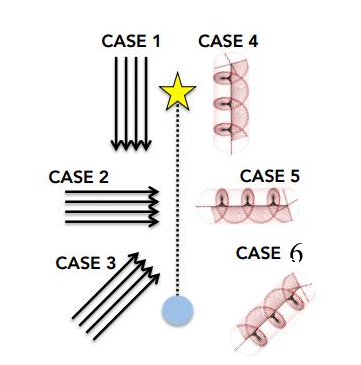
\includegraphics[width=0.3\textwidth]{Bcases.png}
	\caption{Figure reproduced from Long \& Vachaspati (2015)}
\end{figure}
\begin{itemize}
 %\item{Case 0: Random Magnetic field, see section \ref{rmf}}
 \item{Case 1: $\vec{B}_1=- B_0 \hat{z}$}
 \item{Case 2: $\vec{B}_2= B_0 \hat{y}$}
 \item{Case 3: $\vec{B}_3= B_0 \big(\cos(\beta)\hat{y}-\sin(\beta)\hat{z}\big)$}
 \item{Case 4: $\vec{B}_4= B_0\big( \cos(2\pi z/\lambda+\alpha)\hat{y}+\sigma \sin(\cos(2\pi z/\lambda+\alpha)\hat{x}\big)$}
 \item{Case 5: $\vec{B}_5= B_0\big( \cos(2\pi x/\lambda+\alpha)\hat{y}-\sigma \sin(\cos(2\pi x/\lambda+\alpha)\hat{z}\big)$}
 \item{Case 6: $\vec{B}_6= B_0\big( \cos(2\pi s/\lambda+\alpha)\hat{s}_{\perp,1}+\sigma \sin(\cos(2\pi s/\lambda+\alpha)\hat{s}_{\perp,2}\big)$}
\end{itemize}
Here $\beta$ is the orientation angle of the magnetic field in case 3, $\lambda$, $\alpha$ and $\sigma$ are the coherence length, the phase shift and helicity of the magnetic fields
in cases $\{4,5,6\}$. For $\vec{B}_6(\vec{x})$, we introduced $s,\hat{s}_{\perp,1}, \hat{s}_{\perp,2}$ where $s=\vec{x}\cdot\hat{s}$ for some arbitrary chosen $\hat{s}$ while 
\be
\hat{s}_{\perp,1}\cdot \hat{s}_{\perp,2}=\hat{s}_{\perp,1}\cdot \hat{s}=\hat{s}\cdot \hat{s}_{\perp,2}=0.
\ee
To fix $\hat{s}$, the user supplies angles for $theta6,phi6$ and we construct,
\begin{align}
\hat{s}&=\cos(theta6)\hat{z}+\sin(theta6)\cos(phi6)\hat{y}+\sin(theta6)\sin(phi6)\hat{x}\\
\hat{s}_{\perp,1}&=-\hat{s}\times \hat{x}/|\hat{s}\times \hat{x}|\text{  or if ill defined, }\hat{s}_{\perp,1}=\hat{s}\times \hat{y}/|\hat{s}\times \hat{y}|\\
\hat{s}_{\perp,2}&=\hat{s}_{\perp,1}\times \hat{s} 
\end{align}
Setting $theta6=0,~phi6=0$ reduces to case 4.

\subsection{Random Magnetic Field}\label{rmf}
\begin{comment}
A random magnetic field\footnote{
The magnetic field is generated by the procedure outlined in sec II.B of arXiv:1607.00320 (Batista et al.).} centered around the Blazar can be used. One must supply two files, one containing $B(i,j,k)$ at each lattice points and the other
specifying the distance between the lattice points.  This can be done in the UserInput.py file by specifying the $.npy$ file containing these values.
If the files cannot be found but the random magnetic field option is chosen, the program will run but set the magnetic field to 0.\\

To generate the files, one uses the following function in randommagfield.py.
\begin{itemize}
 \item{randommagfield.savemagfield(BoxSize,Lcutoff,helicity=0,info='\_') \tcr{|| Generates the random magnetic field files}}\\
  {\bf{Input}}\\
  -BoxSize: Size of the Box Side in Mpc\\
  -Lcutoff: Size in Mpc between two adjacent lattice points\\
  The box therefore has $(BoxSize/Lcutoff)^3$ number of lattice points\\
  \tcr{Optional Arguments}\\
  -helicity : Set to 0 by default, can be a number between -1 and 1.\\
  -info : Additional information to be tackled to the magnetic field files names.\\
 \newline
 {\bf{Output}}\\
 Two files saved in the $sim\_data/$ directory with names,\\
 'sim\_data/Lcutoff\_'+info\\
 'sim\_data/magfield\_'+info\\
 These can be used in UserInput.py.
\end{itemize}
\end{comment}
It is also possible to use a random magnetic field comprised of modes all having the same magnitude $k_{mag}$. I.e. we can generate a field
\be\label{rmfonemode}
B(\vec{x})=\frac{1}{2M}\sum_{\vec{k}\in K} \vec{B}(\vec{k})e^{i \vec{k}\cdot \vec{x}}
\ee
with the set $K$ being comprised of $2M$ vectors, half of which are isotropically chosen at random with magnitude $k_{mag}$ while the other half insures
a real $B$. For more information on how the Fourier modes are obtained, see the paper.\\
Two options are used to select the vectors. The first is called the ``uniform'' option, here we select $M=2N+1$ vectors approximately uniformely distributed on the sphere. The second option
is called the ``MC'' (for Monte Carlo) option where $M=N$ selects the vector from a uniform random sampling of the sphere.
 Note that this allows more flexibility than specifying a fix case as listed above. The magnetic field used in the code is set by the function named B found in the constraint.py folder.
 Hence changing the function constraint.B will change the magnetic field throughout the code. The function quoted below will do just that, it will set the magnetic field
 to be computed by Eq.~(\ref{rmfonemode}). 
 As this process can be done relatively fast for small $M$, this field can be generate ''on the go`` and is therefore used when generating multiple realization of halo maps. The function we use is,
\begin{itemize}
 \item{stochMorp.setnewB(kmode,Nmodes,helicity,option=1,B0=UserInput.B0) \tcr{|| Sets the magnetic field to be that of Eq (\ref{rmfonemode})}}\\
 {\bf{Input}}\\
  -kmode: float, specifies the norm of the mode k. It also sets the coherence length through $\lambda_c=2\pi/\text{kmode}$.\\
  -Nmodes: Integer, sets the number of modes to use in the set $K$\\
  -helicity: Number between -1 and 1. Setting this to 0 yields a nonhelical magnetic field while 1 or -1 is fully helical.\\
  \tcr{Optional Arguments}\\
  -option: Integer denoting the options 1 or 2 as defined above.
  -option: B0 sets the root mean square value (in Gauss) of the random magnetic field.
 \newline
 {\bf{Output}}\\
 Sets $B$ to be computed from Eq. (\ref{rmfonemode}) in subsequent simulations.
\end{itemize}
 
\section{Useful Functions}

The code contains a large number of functions, most of which have an intermediate use or are simply out of date. In here we tabulate a few functions that should allow one to generalize the
results of \tcr{cite our paper}. The more recent functions usually saves the data in the folder ''sim\_data`` instead of returning it.\\

The main idea was to solve the constraint to find the PP locations and hence the observed photons, then run another function that selected the events in a specified jet.
From this subset of events simulated we applied the functions that would compute the Q-statistics.

\subsection{Event Generation}

\begin{itemize}
\item{EvSim.SimEvent(ds,NumPhotons,cn=1):   \tcr{|| Used to generate events.}} \\
 {\bf{Input}}\\
 -ds : Distance of the source from Earth in Mpc.\\
 -NumPhotons: Number of photons to simulate.\\
 \tcr{Optional Arguments}\\
 -cn: Denotes the file location in which the event will be saved.
 \newline
 {\bf{Output}}\\
 This will create two documents in the folder ''sim\_data/3devents/case(cn)/``\\
 -3devents : Contains NumPhotons entries with the cartesian coordinates of their PP location, $[...,~[x_i,y_i,z_i],~...]$\\
 -3deventsangle : Contains NumPhotons entries with the angular coordinates and energies of the observed photons
 $[...,~[\delta_i-\theta_i,\phi_i,E_i,\theta_i],~...]$\\

 \item{EvSim.JetEvs(NumJets=10,omega=5*gv.degrad,cn=1,doplots=False,jetfix=True):   \tcr{|| Creates a jet and then selects the events in said jet.}} \\
 The jets are randomly generated and have as requirement that at least 3 PP location lie within its openning angle.
 The code makes 20 attempts (I choose this number randomly to insure the code doesn't get stuck) to find a suitable jet.\\
 {\bf{Input}}\\
 -NumJets: Number of jets to find.\\
 -omega: Half-openning angle of the jet.\\
 -cn: Integer of the folder ''sim\_data/3devents/case(cn)/`` that contains the events and where additional files will be generated.\\
 -doplots: Logical variable, if True, creates a 3dplot of the PP locations with the ones in the jets highlighted (the highlightning works poorly).
 The plots are saved as ''3dimg\_(jetnumber)``.\\
 -jetfix: If True, only generate jets that contains Earth in its LOS. If False, randomly select a PP location to be the center of the jet.\\
  {\bf{Output}}\\
 -NumJets images of the observed events under the name ''jetskyimg\_(jetnumber)``.\\
 -Text files named ''jetopenning\_(jetnumber)`` containing the value of omega.\\
 -Text files named ''jetdir\_(jetnumber)`` containing the cartesian coordinates of the unit vector denoting the jet's direction.\\
 -Text files named ''jetcart\_(jetnumber)`` containing the cartesian coordinates of the PP locations intersecting the selected Jet, $[...,~[x_i,y_i,z_i],~...]$\\
 -Text files named ''jetang\_(jetnumber)`` containing the  the angular coordinates and energies of the observed photons due to the jet, 
 $[...,~[\delta_i-\theta_i,\phi_i,E_i,\theta_i],~...]$\\
 
  \item{EvSim.SimNHalos(N=2,kmode=kmode,Nmodes=Nmodes,hel=helicity,cns=100,\\
  njets=njets,Nphotons=Nphotons,MCB=False,B0=UI.B0,UseUIBins=True,\\
  case=False,jetfix=True,CalcBcB=False,CQ=0,omega=5*gv.degrad):   \tcr{|| Generates N simulations and saves the data in ''sim\_data/3devents/case(number)/``}} \\
 {\bf{Input}}\\
 -N: Number of simulations to generate.\\
 -cns: Integer of the first folder ''sim\_data/3devents/case(cns)/`` that contains the events and where additional files will be generated.\\
 -njets: Number of jets to find.\\
 -Nphotons: number of photons to simulate in each realization\\
 -omega: Half-openning angle of the jet.\\
 -B0: Sets the root mean square of the magnetic field in Gauss.\\
 -kmode: float, specifies the norm of the mode k. It also sets the coherence length through $\lambda_c=2\pi/\text{kmode}$.\\
 -Nmodes: Integer, sets the number of modes to use in the set $K$\\
 -hel: Number between -1 and 1. Setting this to 0 yields a nonhelical magnetic field while 1 or -1 is fully helical.\\
 -jetfix: If True, only generate jets that contains Earth in its LOS. If False, randomly select a PP location to be the center of the jet.\\
 -CQ: Integer (0 or 1 as of this writing), CQ=0 (1) computes the Q-statistic without (with) the Heaviside function.\\
 -UseUIBins: if True, the energy bins used to compute Q are the ones supplied in the UserInput.py file. If False, the bins are automatically set by dividing the observed photons in 3 bins.
 -MCB: Logical, if True, uses the ''MC`` method to generate the random magnetic fields (i.e. option 2). We use option 1 if False. (see Sec~\ref{rmf} for details about the options)\\
 -case: Integer, if not False, this selects the magnetic field as defined by case (number) to be used. \\
 -CalcBcB: if True, computes $\langle {\bf B}\cdot \nabla \times B\rangle _{LOS}$ along the jet's LOS and outputs a plot in ''/case(number)/''\\
  {\bf{Output}}\\
 $N$ files in the folder  'sim\_data/3devents`` (see the description of ''cns''). The files contain the output of JetEvs and SimEvent. 
 They also contain the Q statistics of every halo created by the $i^{th}$ jet and $j^{th}$ energy bin in the file named ``Q\_i\_bin\_j.txt'' .
 The energy ranges of each bins are stored in the file ``UsedEbins.txt'' and the angular region $R$ used as the x-axis of the Q values are
 stored in ``region\_i.txt''.


\begin{comment}
 \item{qstatistics.genevents(ntsr,NumPhotons,ds=UserInput.dS,phi=0,omega=np.pi,alpha=0,jetact=0)   \tcr{|| Used to generate events.}} \\
 {\bf{Input}}\\
 -ntsr: Noise to Signal ratio of background isotropic events to blazar events, ntsr=0 implies no background events.\\
 -NumPhotons: Number of photons to simulate.\\
 \tcr{Optional Arguments}\\
 -alpha: Angle of the jet with respect to Earth (alpha=0 $\implies$ jet points at earth).\\
 -phi: Angle of the jet in the azimuthal angle.\\
 -Omega: Openning angle of the jet (photons must lie within an angle of Omega of the direction set by alpha and phi).\\
 -ds: Distance of the source from Earth in Mpc.\\
 -jetact: Jet=1 or no Jet=0 (isotropic emission).\\
 \newline
 {\bf{Output}}\\
 evtot,evBlazar,evback,evtotC,evBlazarC,evbackC\\
 -evtot: Array of all events binned per energy bins according to UserInput.EBins. $\text{evtot}[i]=[...,[\theta_i,\phi_i],...]$ for bin $i$.\\
 -evBlazar: Same format as evtot, only contains Blazar events.\\
 -evback: Same format as evtot, only contains background events.\\
 -evtotC: Same format as evtot, with cartesian coords of the events unit vector. $\text{evtot}[i]=[...,[x_i,y_i,z_i],...]$\\
 -evBlazarC: Same format as evtotC, only contains Blazar events.\\
 -evbackC: Same format as evtotC, only contains background events.\\
 \end{comment}
 
 \item{stochMorp.stomorp(ds,NumPhotons,phi=0,omega=np.pi,alpha=0,LeptonId=False) \tcr{|| OLD AND LIMITED. We keep it as it can track the sign of the lepton producing the observed events. The Jet variables are only important when jetactivated=1 in the UserInput.py file.}} \\
 {\bf{Input}}\\
 -ds: Distance of the source from Earth in Mpc.\\
 -NumPhotons : Number of photons to simulate.\\
 \tcr{Optional Arguments}\\
 -alpha: Angle of the jet with respect to Earth (alpha=0 $\implies$ jet points at earth).\\
 -phi: Angle of the jet in the azimuthal angle.\\
 -Omega: Openning angle of the jet (photons must lie within an angle of Omega of the direction set by alpha and phi).\\
 -LeptonId : if True, keep track of the charge $q=\pm 1$ of the lepton that upscattered the observed photon. If False, we return $q=1$ for all events. \\
 \newline
 {\bf{Output}}\\
 tcospsol,tsinpsol,events\\
 -events: Array of events with $[...,[\theta_i,\phi_i,E_i,q_i],...]$\\
 -tcospsol: Array of simulated event with $[...,\frac{\theta_i}{degrad}\cos\phi_i,...]$\\
 -tsinpsol: Array of simulated event with $[...,\frac{\theta_i}{degrad}\sin\phi_i,...]$


\end{itemize}



\subsection{Plotting and visualization functions}

\begin{itemize}
 \item{stochMorp.plotStoMorp(figname,phi=0,omega=np.pi,alpha=0,NumEvents=1000,Morp=False,LeptonId=False) \tcr{|| Plots Blazar emission.}}\\
 \tcr{If no angles are supplied, the code assumes an isotropic emission from the Blazar. The code also assumes that the distance of the Blazar to 
 earth is given by the global variable UserInput.dS .}\\
 {\bf{Input}}\\
 -figname: Name of the figure, example figname='test'\\
 \tcr{Optional Arguments}\\
 -alpha: Angle of the jet with respect to Earth (alpha=0 $\implies$ jet points at earth).\\
 -phi: Angle of the jet in the azimuthal angle.\\
 -Omega: Openning angle of the jet (photons must lie within an angle of Omega of the direction set by alpha and phi).\\
 -NumEvents: Number of Photons to simulate.\\
 -Morp : If True, also draw the expected morphology if no randomness in the MFP exists. This option can work poorly for certain magnetic field choices (such as a stochastic one).\\
 -LeptonId : If True, color code the events by positron (red) and electron (black) instead of energy bins.\\
 {\bf{Output}}\\
 Saves a figure in the $imgs/$ directory as figname
 \item{stochMorp.plotevs(figname,ev) \tcr{|| Plot some event array ev}}\\
 {\bf{Input}}\\
 -figname: Name of the figure, example figname='test'\\
 -ev : Numpy array of events arranged by energy bins. Format as outputed by qstatistics.genevents: $ev[i,j]=[\theta_{i,j},\phi_{i,j}]$, i:Number of Ebins, j:Number of Event.\\
 {\bf{Output}}\\
 Saves a figure in the $imgs/$ directory as figname\\
 \end{itemize}

\subsection{Q-statistics}
\begin{itemize}
 \item{qstatistics.analyzeq(evtot,evBl=False,evMc=False) \tcr{|| Computed Q out of events.}}\\
  {\bf{Input}}\\
  evtotC: Total event file as output in genevents. \\
 \tcr{Optional Arguments}\\
 evBl: Blazar event file as output in genevents. If not passed, the output for Qbla is an array of 0. \\
 evMc: Background event file as output in genevents. If not passed, the output for Qmc is an array of 0. \\
     \newline
 {\bf{Output}}\\
 Qtot,Qbla,Qmc\\
 Qtot: Q-stats for total events. \\
 Qbla: Q-stats for blazar events. \\
 Qmc: Q-stats for background events. \\
 The output have the same format: Q[i,j,k] with $i$ being the energy pair number, $j=\{0,1\}$ being the mean and standard deviation to $Q$'s contribution from each HE photons, $k$ being the index of the radius surveyed.
 \begin{comment}
 \item{qstatistics.qstats(numruns,ntsr,NumPhotons,totalonly=False) \tcr{|| Statistics of Q over many realizations.}}\\
 {\bf{Input}}\\
 numruns: Number of realizations\\
 ntsr: Noise to Signal ratio of background isotropic events to blazar events, ntsr=0 implies no background events.\\
 NumPhotons: Number of Photons simulated in the Blazar.\\
 \tcr{Optional Arguments}\\
  totalonly: If True, ignores the input of evBlazarC and evbackC and only computes Q-statistics for evtotC.
     \newline
 {\bf{Output}}\\
 Qtot,Qbla,Qmcmc\\
 Same format as the ouput for qstatistics.analyzeq(...) described above. The only difference is that the $j$ variable now labels the mean
 and standard deviations of the $Q$'s over the multiple realizations.
 \end{comment}
 \item{qstatistics.plotq(figname,Qtot,Qbla=False,Qmc=False): \tcr{|| Plots the Q's }}\\
 {\bf{Input}}\\ 
 figname: Name of the figure, example figname='test'
 Qtot: Same format as outputted by qstats or qanalyze. The error bars are created using the value stored in the $j=1$ index.\\
 \tcr{Optional Arguments}\\
 Qbla,Qmc: Same format as outputted by qstats or qanalyze. The error bars are created using the value stored in the $j=1$ index. If these arrays are not passed to the function, we do not plot them.
     \newline
 {\bf{Output}}\\
 Saves a figure in the $imgs/$ directory as figname\\
  Creates figures such as in fig \ref{qplotex}.
 \begin{comment}
  \item{qstatistics.plotNTSReffect(figname,numruns,ntsrMIN,ntsrMAX,numsteps,NumPhotons) \tcr{|| Plots the Q's }}\\
   Plots the Q-statistics but now changes the ntsr from ntsrMIN to ntsrMAX in numsteps. The input are described above.
   Outputs a figure in the $imgs/$ directory as figname. Creates figures such as in fig \ref{qplotex} (right side)
   \end{comment}
   \begin{figure}[tbhp]
	\centering
	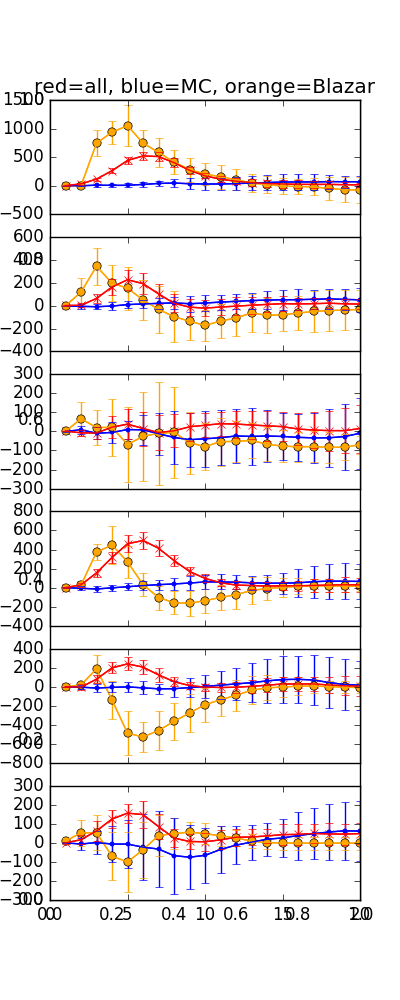
\includegraphics[width=0.3\textwidth]{qplotex1.png}
%	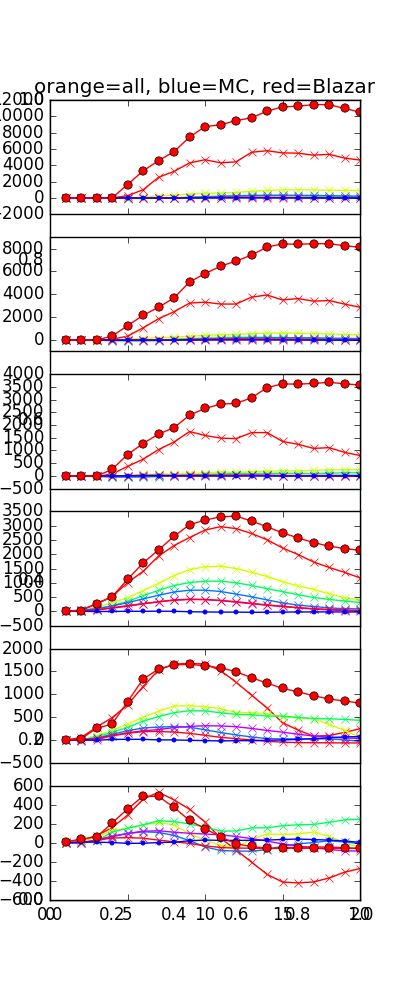
\includegraphics[width=0.3\textwidth]{qplotex2.png}
	\caption{q-stats figures. Labels, legends and titles might change in the future (for instance the title on the right figure is wrong but has then
	been fixed in the code).}\label{qplotex}
    \end{figure}
 \end{itemize}
 
 
\item{EvSim.QsPlot(N=2,cns=100,name='_',plotallQ=True,plotinCN=False,
    Qstart='Q_',EvsList=False,labelEbins=True,evsSP=False)}\\
    {\bf{Input}}\\
 QfromEvs
 Qhist
 Qplot

\end{document}
